\section{Mô đun quản lý cơ sở dữ liệu}
Bộ CSDL ảnh phục vụ cho huấn luyện và tinh chỉnh các mô hình phân loại trong các thuật toán Học sâu nói riêng và Học máy nói chung là thành phần vô cùng quan trọng, quyết định chủ yếu đến độ chính xác mà mô hình đạt được. Do vậy, chúng cần được lưu trữ và quản lý một cách khoa học. Trong hệ thống lưu trữ, bộ CSDL ảnh huấn luyện được chia thành các thư mục riêng biệt:
\begin{itemize}
	\item {\bf Thư mục ảnh gốc}: Là bộ ảnh ban đầu được sử dụng để xây dựng phiên bản mô hình phân loại đầu tiên, gồm các thư mục con được phân loại chính xác là ảnh gốc.
	\item {\bf Thư mực ảnh thực tế chưa duyệt}: Là các ảnh được gửi thực tế do trình duyệt của người phân loại gửi lên để thực hiện phân loại, được chia thành các thư mục con tương ứng với 2 loại nhãn có lao hay không có lao như mô hình đã được huấn luyện. Các ảnh này chưa được kiểm duyệt và chưa được sử dụng để tăng cường cho CSDL ảnh huấn luyện.
	\item {\bf Thư mục ảnh thực tế đã duyệt}: Bao gồm các ảnh thực tế đã được kiểm duyệt đảm bảo chất lượng tốt và loại nhãn ảnh được gán là hợp lệ, những ảnh này đã được gán nhãn đúng, chuyển tới các thư mục con tương ứng và sẽ được sử dụng để huấn luyện tăng cường cho mô hình phân loại ban đầu. Các thư mục ảnh này đều được đặt trong các thư mục cha được đánh số ứng với phiên bản mô hình được huấn luyện bổ sung, nhằm đảm bảo không có sự nhầm lẫn giữa các phiên bản với nhau.
\end{itemize}

\section{Bộ huấn luyện mô hình}
Nằm ở tầng thứ tư trong kiến trúc n tầng của hệ thống, bộ huấn luyện mô hình là thành phần có vai trò quan trọng hàng đầu, chịu toàn bộ trách nhiệm về các mô hình phân loại từ giai đoạn khởi tạo đến tinh chỉnh và hoàn thiện, cũng như quản lý và đánh giá độ chính xác các phiên bản khác nhau của mô hình. Bộ huấn luyện được cài đặt và triển khai thành một mô đun hoàn toàn tách biệt với các thành phần còn lại của server, giúp cho việc nâng cấp hay thay thế có thể thực hiện độc lập mà không gây ảnh hưởng đến hoạt động thông thường của server. Các ca sử dụng chính của mô đun bao gồm: Cấu hình CSDL ảnh để huấn luyện, Xác định các tham số cho mô hình huấn luyện, Thực hiện huấn luyện và Xuất ra mô hình đã huấn luyện xong theo phiên bản tương ứng với bộ CSDL ảnh đã sử dụng (hình \ref{fig:usecase_bo_huan_luyen}).
\begin{figure}[H]
	\centering
	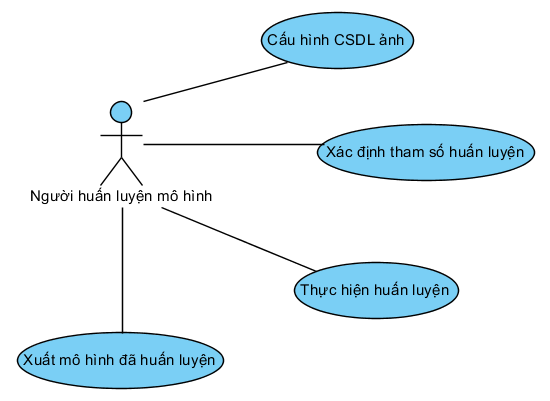
\includegraphics[width=0.9\linewidth]{images/usecase_bo_huan_luyen}
	\caption{Biểu đồ usecase của Bộ huấn luyện mô hình.}
	\label{fig:usecase_bo_huan_luyen}
\end{figure}
Đặc tả biểu đồ usecase bộ huấn luyện mô hình:\\

\subsection{Cấu hình CSDL ảnh:}
\begin{itemize}
	\item Mục đích: Cấu hình các thông tin cơ bản về CSDL ảnh cho bộ huấn luyện mô hình, như: đường dẫn thư mục lưu ảnh, phiên bản huấn luyện hiện tại, số lượng ảnh huấn luyện và ảnh test…
	\item Tác nhân, Mô tả chung:
	\begin{itemize}
		\item Tác nhân: Người quản trị hệ thống, hoặc người quản trị mô đun huấn luyện mô hình phân loại.
		\item Mô tả chung: Người quản trị khi muốn bắt đầu huấn luyện mới, hoặc huấn luyện bổ sung cho mô hình phân loại thì trước hết cần cấu hình thông tin bộ CSDL ảnh phục vụ cho huấn luyện.
	\end{itemize}
	\item Luồng sự kiện chính: Người quản trị cập nhật thông tin về bộ CSDL ảnh trong file cấu hình cho bộ huấn luyện, tạo mới các file ghi lại đường dẫn đến ảnh huấn luyện, ảnh test và nhãn đánh dấu tương ứng.
	\item Luồng thay thế: Không.
	\item Các yêu cầu cụ thể: Thông tin bộ CSDL ảnh phải chính xác, đường dẫn đến vị trí ảnh huấn luyện và ảnh test phải hợp lệ.
	\item Điều kiện trước: Bộ CSDL ảnh huấn luyện phải có sẵn trong hệ thống lưu trữ, các ảnh đã được duyệt và đặt đúng thư mục tương ứng.
	\item Điều kiện sau: Không.
\end{itemize}

\subsection{Xác định tham số huấn luyện:}
\begin{itemize}
	\item Mục đích: Tính toán các thông số cần thiết từ bộ CSDL ảnh và xác định các	tham số nhằm định nghĩa mô hình và cách thức huấn luyện mô hình.
	\item Tác nhân, Mô tả chung:
	\begin{itemize}
		\item Tác nhân: Người quản trị hệ thống, hoặc người quản trị mô đun huấn luyện mô hình phân loại.
		\item Mô tả chung: Người quản trị khi muốn bắt đầu thực hành huấn luyện	mới, hoặc huấn luyện bổ sung cho mô hình phân loại thì cần phải xác định các tham số định nghĩa quá trình huấn luyện cũng như các giá trị cần thiết liên quan đến bộ CSDL ảnh.	
	\end{itemize}
	\item Luồng sự kiện chính: Người quản trị gọi file thực thi các hàm tính toán giá trị liên quan đến bộ CSDL ảnh đầu vào, sửa đổi cập nhật tham số trong các file định nghĩa huấn luyện mô hình.
	\item Luồng thay thế: File thực thi tính toán thông báo lỗi khi không thể tính toán	thành công trên bộ CSDL ảnh đã cấu hình.
	\item Các yêu cầu cụ thể: Đầu ra của file thực thi tính toán phải là các file dữ liệu theo định dạng chuẩn, các tham số định nghĩa mô hình phải phù hợp với mục	đích huấn luyện.
	\item Điều kiện trước: Các thông tin liên quan đến bộ CSDL ảnh phải được cấu hình hợp lệ trước đó.
	\item Điều kiện sau: Thông báo tính toán thành công giá trị cần thiết từ bộ CSDL ảnh.
\end{itemize}

\subsection{Thực hiện huấn luyện:}
\begin{itemize}
	\item Mục đích: Huấn luyện, tinh chỉnh mô hình phân loại cho hệ thống sử dụng bộ CSDL ảnh trên nền một mô hình đã huấn luyện trước. Ảnh được sử dụng để huấn luyện có thể là các ảnh ban đầu, gồm ảnh gốc và ảnh sinh tự động, hoặc là các ảnh được thu thập, lưu trữ trong quá trình người phân loại gửi yêu cầu phân loại lên server.
	\item Tác nhân, Mô tả chung:
	\begin{itemize}
		\item Tác nhân: Người quản trị hệ thống, hoặc người quản trị mô đun huấn luyện mô hình phân loại.
		\item Mô tả chung: Người quản trị khi đã hoàn thành việc thu thập ảnh, cấu hình các thông tin liên quan đến CSDL ảnh cũng như tính toán, xác định các tham số cần thiết thì có thể bắt đầu thực hiện huấn luyện mô hình phân loại cho hệ thống.
	\end{itemize}
	\item Luồng sự kiện chính: Người quản trị gọi file thực thi các câu lệnh cần thiết để bắt đầu huấn luyện mô hình. Các câu lệnh được chia thành hai loại: Câu lệnh	bắt đầu một phiên huấn luyện mới và Câu lệnh tiếp tục phiên huấn luyện bị tạm dừng trước đó.
	\item Luồng thay thế: File thực thi thông báo lỗi khi không thể thực hiện huấn luyện với các tham số đầu vào đã cấu hình, gồm tham số về file định nghĩa mô hình, mô hình được huấn luyện trước, lựa chọn sử dụng card đồ họa GPU, hoặc file trạng thái huấn luyện tại thời điểm tạm dừng (trong trường hợp tiếp tục phiên huấn luyện chưa hoàn thành)…
	\item Các yêu cầu cụ thể: Đầu ra của quá trình huấn luyện là một mô hình phân loại và các file ghi lại nhật ký huấn luyện, gồm các thông tin, cảnh báo hoặc lỗi xảy ra trong quá trình huấn luyện để người quản trị có thể truy vết nếu cần thiết. Ngoài ra, thông tin về phiên bản của mô hình phân loại được huấn luyện cũng được lưu lại.
	\item Điều kiện trước: Thông tin cấu hình CSDL ảnh và tham số định nghĩa mô	hình huấn luyện phải chính xác. Mô hình được huấn luyện trước và file trạng thái huấn luyện tại thời điểm tạm dừng phải hợp lệ.
	\item Điều kiện sau: Thông báo huấn luyện thành công mô hình, với một số thông tin cơ bản của phiên huấn luyện như phiên bản hiện tại của mô hình và độ	chính xác đạt được.
\end{itemize}

\subsection{Xuất mô hình đã huấn luyện}
\begin{itemize}
	\item Mục đích: Xuất ra mô hình đã được huấn luyện thành công, làm đầu vào cho	mô đun tính toán phân loại của server.
	\item Tác nhân, Mô tả chung:
	\begin{itemize}
		\item Tác nhân: Người quản trị hệ thống, hoặc người quản trị mô đun huấn luyện mô hình phân loại.
		\item Mô tả chung: Sau khi người quản trị đã hoàn thành việc huấn luyện	mô hình, để mô hình mới có thể được sử dụng vào quá trình tính toán	phân loại thực tế người quản trị phải xuất mô hình ra và thay thế cho	mô hình cũ.
	\end{itemize}
	\item Luồng sự kiện chính: Người quản trị gọi file thực thi câu lệnh xuất mô hình đã huấn luyện ra thư mục lưu trữ (đã cài đặt trong file cấu hình chung của hệ thống). Mô hình cũ đang được sử dụng được chuyển sang thư mục lưu các phiên bản không còn sử dụng.
	\item Luồng thay thế: File thực thi thông báo lỗi trong quá trình xuất mô hình đã huấn luyện và chuyển mô hình phiên bản cũ sang thư mục để lưu trữ.
	\item Các yêu cầu cụ thể: Không.
	\item Điều kiện trước: Mô hình đã được huấn luyện phải là mô hình hoàn thiện. Các thông tin cấu hình về thư mục mô hình hiện tại và thư mục lưu trữ các mô hình với phiên bản thấp hơn phải hợp lệ.
	\item Điều kiện sau: Thông báo xuất mô hình thành công.
\end{itemize}

\section{Các mô đun phía Server}
Chương trình phía server được cấu thành bởi các nhiều mô đun, đảm nhiệm các vai trò nhiệm vụ khác nhau liên quan đến huấn luyện, quản lý mô hình phân loại, cấu hình giao thức giao tiếp giữa client và server hay xử lý logic đa luồng, đảm bảo khả năng tính toán cho nhiều yêu cầu cùng lúc… Các ca sử dụng tương ứng với các nhiệm vụ này được thể hiện trong Hình 3.8 cùng với phần mô tả cụ thể bên dưới.
\begin{figure}[H]
	\centering
	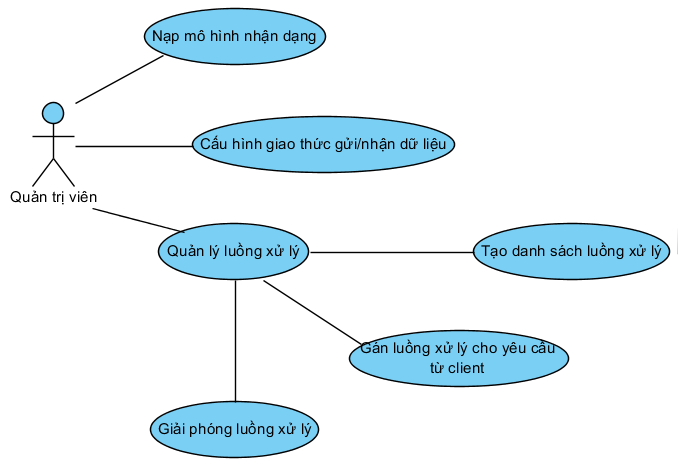
\includegraphics[width=1\linewidth]{images/usecase_server}
	\caption{Biểu đồ usecase của Server.}
	\label{fig:usecase_server}
\end{figure}
Đặc tả biểu đồ:
\subsection{Nạp mô hình phân loại}
\begin{itemize}
	\item Mục đích: Nạp vào hệ thống mô hình phân loại phiên bản mới nhất được xuất ra bởi mô đun Bộ huấn luyện mô hình, phục vụ cho việc xử lý các yêu cầu nhận được từ ứng dụng phía client sau đó.
	\item Tác nhân, Mô tả chung:
	\begin{itemize}
		\item Tác nhân: Người quản trị hệ thống.
		\item Mô tả chung: Để hệ thống có thể thực hiện tính toán và phân loại nhãn của ảnh do ứng dụng client gửi lên, mô hình phân loại cần phải	được nạp trước vào hệ thống. Việc nạp mô hình này chỉ thực hiện một lần tại thời điểm bắt đầu một phiên chạy của server.
	\end{itemize}
	\item Luồng sự kiện chính: Người quản trị khởi động chương trình server, hàm khởi tạo của chương trình tự động gọi câu lệnh thực thi việc nạp mô hình phân loại.
	\item Luồng thay thế: Chương trình server thông báo không nạp mô hình phân loại	thành công, với thông tin cụ thể về lỗi xảy ra, như file định dạng chế độ triển khai của mô hình hoặc mô hình phân loại không hợp lệ.
	\item Các yêu cầu cụ thể: Phiên bản mô hình phân loại là phiên bản hoàn thiện mới nhất. Các thông tin cấu hình cho chương trình server phải hợp lệ.
	\item Điều kiện trước: Các thư viện cần thiết cho chương trình server đã được cài đặt đầy đủ và đúng phiên bản được khuyến cáo.
	\item Điều kiện sau: Thông báo nạp mô hình thành công.
\end{itemize}

\subsection{Cấu hình giao thức gửi/nhận dữ liệu:}
\begin{itemize}
	\item Mục đích: Cấu hình các thông tin quyết định giao thức gửi, nhận dữ liệu giữa chương trình server và ứng dụng phía client, ví dụ: giao thức HTTP, cổng kết	nối…
	\item Tác nhân, Mô tả chung:
	\begin{itemize}
		\item Tác nhân: Người quản trị hệ thống.
		\item Mô tả chung: Người quản trị khi muốn khởi động chương trình server để nhận các yêu cầu từ ứng dụng client và gửi trả kết quả phân loại	thì phải cấu hình giao thức gửi, nhận dữ liệu để thống nhất cách thức giao tiếp giữa hai thành phần server và client. Việc cấu hình này này	chỉ thực hiện một lần tại thời điểm bắt đầu một phiên chạy của server.
	\end{itemize}	
	\item Luồng sự kiện chính: Người quản trị khởi động chương trình server, hàm khởi tạo của chương trình tự động gọi câu lệnh thực thi việc cấu hình các thông số cho giao thức gửi, nhận dữ liệu giữa server và ứng dụng phía client.
	\item Luồng thay thế: Chương trình server thông báo không thể cấu hình được giao thức gửi, nhận dữ liệu, với thông tin cụ thể về lỗi xảy ra.
	\item Các yêu cầu cụ thể: Các thông tin của giao thức gửi, nhận dữ liệu phải hợp lệ, cổng giao tiếp phải ở trạng thái tự do, không bị tranh chấp với các chương	trình khác.
	\item Điều kiện trước: Các thư viện cần thiết cho chương trình server đã được cài đặt đầy đủ và đúng phiên bản được khuyến cáo. Chương trình server đã nạp thành công mô hình phân loại.
	\item Điều kiện sau: Thông báo cấu hình thành công giao thức gửi, nhận dữ liệu với các thông tin cụ thể của giao thức
\end{itemize}

\subsection{Tạo danh sách luồng xử lý}
\begin{itemize}
	\item Mục đích: Khởi tạo trước một loạt các luồng xử lý, nhằm phục vụ quá trình	tách riêng tính toán và phân loại cho từng yêu cầu phía client trong suốt phiên chạy của chương trình server.
	\item Tác nhân, Mô tả chung:
	\begin{itemize}
		\item Tác nhân: Người quản trị hệ thống.
		\item Mô tả chung: Trong quá trình chạy, để đảm bảo chương trình không bị chậm trễ khi đồng thời có nhiều yêu cầu từ các client khác nhau, chương trình server cần thực hiện việc xử lý này theo phương pháp đa	luồng. Nghĩa là: mỗi yêu cầu từ phía client được xử lý trên một luồng
		riêng, không bị ảnh hưởng và không gây ảnh hưởng đến các luồng xử lý khác. Để thuận tiện cho việc quản lý và tránh tình trạng tràn bộ nhớ do quản lý luồng không tốt, chương trình khởi tạo trước danh sách một loạt các luồng xử lý và sử dụng cờ trạng thái để giao việc cũng như giải phóng luồng.
	\end{itemize}
	\item Luồng sự kiện chính: Người quản trị khởi động chương trình server, hàm khởi tạo của chương trình tự động gọi câu lệnh thực thi việc khởi tạo danh sách	một loạt các luồng xử lý. Số lượng luồng xử lý được lưu dưới dạng hằng số trong file cấu hình chung của hệ thống.
	\item Luồng thay thế: Chương trình server thông báo không thể khởi tạo thành công các luồng xử lý.
	\item Các yêu cầu cụ thể: Không.
	\item Điều kiện trước: Các thư viện cần thiết cho chương trình server đã được cài đặt đầy đủ và đúng phiên bản được khuyến cáo. Chương trình server đã hoàn thành các bước Nạp mô hình huấn luyện và Cấu hình giao thức gửi, nhận dữ	liệu.
	\item Điều kiện sau: Thông báo tạo thành công danh sách các luồng xử lý.
\end{itemize}

\subsection{Gán luồng xử lý cho yêu cầu từ phía Client:}
\begin{itemize}
	\item Mục đích: Gán việc tính toán xử lý cho mỗi yêu cầu từ ứng dụng phía client cho một luồng xử lý đang ở trạng thái rảnh rỗi, nhằm hạn chế tối đa khả năng gây chậm trễ cho ứng dụng khi phải xử lý cùng lúc nhiều yêu cầu.
	\item Tác nhân, Mô tả chung:
	\begin{itemize}
		\item Tác nhân: Thành phần xử lý logic quản lý luồng trong chương trình	server.
		\item Mô tả chung: Mỗi khi có yêu cầu mới từ phía client, đầu tiên server phải kiểm tra trạng thái tính toán của các luồng xử lý trong danh sách được khởi tạo từ ban đầu. Nếu có một luồng xử lý đang ở trạng thái	rỗi, server gán luồng xử lý này cho yêu cầu mới nhận để luồng xử lý thực hiện các phép tính toán, phân loại và trả về kết quả cho client tương ứng. Nếu toàn bộ các luồng xử lý này đều ở trạng thái đang tính toán thì yêu cầu được đưa vào một hàng đợi, đợi đến khi có một luồng xử lý được giải phóng và đặt trạng thái rảnh rỗi.
	\end{itemize}
	\item Luồng sự kiện chính: Thành phần xử lý logic quản lý luồng xử lý kiểm tra danh sách các luồng xử lý, gán yêu cầu mới nhận được cho một luồng xử lý rảnh rỗi.
	\item Luồng thay thế: Nếu không có luồng xử lý nào trong danh sách đang ở trạng	thái rảnh rỗi, yêu cầu được đưa vào hàng đợi và sẽ được xử lý tiếp khi có một luồng xử lý hoàn thành việc tính toán trước đó.
	\item Các yêu cầu cụ thể: Trong danh sách luồng xử lý còn ít nhất một luồng ở trạng	thái rảnh rỗi.
	\item Điều kiện trước: Các luồng xử lý phải được khởi tạo thành công từ khi bắt	đầu chạy chương trình server.
	\item Điều kiện sau: Thông báo gán luồng xử lý thành công.
\end{itemize}

\subsection{Giải phóng luồng xử lý}
\begin{itemize}
	\item Mục đích: Cập nhật trạng thái của luồng xử lý khi đã hoàn thành việc tính	toán và phân loại cho yêu cầu được giao.
	\item Tác nhân, Mô tả chung:
	\begin{itemize}
		\item Tác nhân: Thành phần xử lý logic quản lý luồng trong chương trình	server.
		\item Mô tả chung: Khi luồng xử lý hoàn thành việc tính toán, phân loại và gửi kết quả về cho phía client, luồng cần được giải phòng bằng cách cập nhật lại trạng thái của luồng thành trạng thái rảnh rỗi. Luồng xử lý tiếp tục đợi đến khi được giao cho một yêu cầu phân loại mới từ server.
	\end{itemize}
	\item Luồng sự kiện chính: Thành phần xử lý logic quản lý luồng xử lý cập nhật trạng thái của một luồng thành trạng thái rỗi khi luồng đó thông báo hoàn thành việc xử lý yêu cầu được giao trước đó.
	\item Luồng thay thế: Không.
	\item Các yêu cầu cụ thể: Thành phần xử lý logic quản lý luồng xử lý cần phải có cơ chế để nhận được thông báo hoàn thành tính toán từ các luồng trong danh sách.
	\item Điều kiện trước: Các luồng xử lý phải được khởi tạo thành công từ khi bắt	đầu chạy chương trình server. Luồng xử lý đã hoàn thành tính toán và đưa ra thông báo tới thành phần quản lý logic luồng trong chương trình.
	\item Điều kiện sau: Thông báo luồng xử lý đã hoàn thành tính toán. Thành phần quản lý luồng xử lý cập nhật trạng thái của luồng thành trạng thái rảnh rỗi. Sau đó, thành phần quản lý luồng tiếp tục kiểm tra hàng đợi các yêu cầu từ client chưa được xử lý, nếu hàng đợi không rỗng thì lấy yêu cầu đầu tiên từ	hàng đợi và gán cho luồng xử lý đang rảnh rỗi.
\end{itemize}

\section{Ứng dụng phía Client}
Ứng dụng phía Client là ứng dụng trên trình duyệt, là một thành phần trong hệ thống đảm nhiệm vai trò thu thập ảnh đầu vào để phân loại, gồm các chức năng chính sau đây: Chọn ảnh từ thư viện và Xem kết quả phân loại do mô đun phía Server trả về. Ngoài ra, ứng dụng còn có các chức năng phụ khác, như: Phàn hồi kết quả, Xem thông tin về ứng dụng hoặc hướng dẫn sử dụng ứng dụng.
\begin{figure}[H]
	\centering
	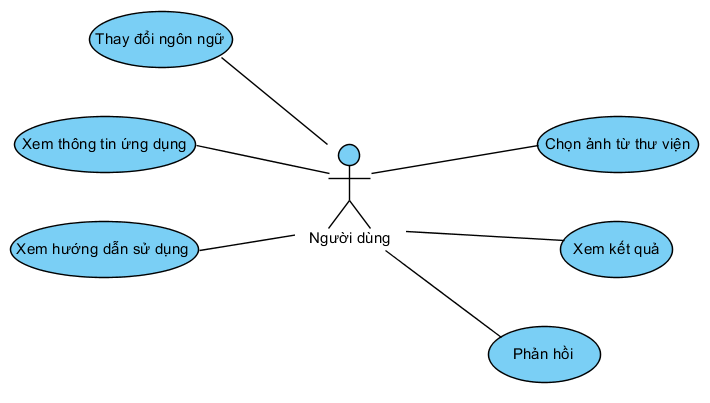
\includegraphics[width=1\linewidth]{images/usecase_client}
	\caption{Biểu đồ usecase của Client.}
	\label{fig:usecase_client}
\end{figure}
\subsection{Chọn ảnh trong thư viện ảnh}
\begin{itemize}
	\item Mục đích: Lấy ra một ảnh đã chụp trong thư viện ảnh trên máy tính để gửi lên cho server, yêu cầu tính toán phân loại.
	\item Tác nhân, Mô tả chung:
	\begin{itemize}
		\item Tác nhân: Người phân loại ứng dụng.
		\item Mô tả chung: Khi người phân loại muốn thực hiện phân loại một ảnh nào đó, nhưng tại thời điểm đó người phân loại không có kết nối mạng để kết nối tới server, người phân loại có thể lưu lại ảnh	trong thư viện ảnh của máy tính và thực hiện việc phân loại sau đó.
	\end{itemize}	
	\item Luồng sự kiện chính: Người phân loại chọn một ảnh đã lưu trong thư viện ảnh, ứng dụng thực hiện mã hóa và nén dữ liệu ảnh rồi gửi lên server, đồng thời hiển thị thông báo cho người phân loại chờ kết quả phân loại.
	\item Luồng thay thế: Ứng dụng không thể truy cập vào thư mục thư viện ảnh của máy tính, hoặc thông báo lỗi không thể kết nối đến chương trình server.
	\item Các yêu cầu cụ thể: Không.
	\item Điều kiện trước: Ứng dụng đã được khởi động thành công, các thông tin ảnh có sẵn.
	\item Điều kiện sau: Thông báo người phân loại chờ trong lúc chương trình server thực hiện tính toán phân loại.
\end{itemize}

\subsection{Xem kết quả}
\begin{itemize}
	\item Mục đích: Hiển thị kết quả phân loại ảnh nhận được từ chương trình server. Kết quả hiển thị cho người phân loại bao gồm một kết quả phân loại cao nhất đi kèm với tỉ lệ phần trăm dự đoán của mô hình giúp người phân loại tham khảo, đồng thời phục vụ cho tính năng	phản hồi kết quả khi thông tin phân loại bị sai lệch.
	\item Tác nhân, Mô tả chung:
	\begin{itemize}
		\item Tác nhân: Ứng dụng phía client.
		\item Mô tả chung: Sau khi chương trình server nhận được yêu cầu từ phía client, server thực hiện tính toán trên luồng xử lý và trả về kết quả cho ứng dụng phía client. Lúc này ứng dụng sẽ hiển thị kết quả nhận được cho người cần thực hiện phân loại.
	\end{itemize}	
	\item Luồng sự kiện chính: Ứng dụng hiển thị cho người phân loại kết quả phân loại, gồm dự đoán kết quả phân loại kèm phần trăm dự đoán.
	\item Luồng thay thế: Ứng dụng hiển thị kết quả là các chuỗi ký tự vô nghĩa, nguyên	nhân do quá trình nhận và bóc tách dữ liệu từ server bị lỗi. 
	\item Các yêu cầu cụ thể: Không.
	\item Điều kiện trước: Ứng dụng đã gửi ảnh lên server và đang ở trạng thái đợi kết quả tính toán phân loại từ server.
	\item Điều kiện sau: Ứng dụng sẽ hiển thị thành công kết quả nhận được cho người phân loại.
\end{itemize}